El comercio electrónico se refiere al proceso de compra o venta de productos o servicios a través de Internet. Las compras en línea se están volviendo cada vez más populares debido a la velocidad y facilidad de uso para los clientes. Las actividades de comercio electrónico, como la venta en línea, pueden dirigirse a consumidores u otras empresas. Vender en línea puede ayudar a su empresa a llegar a nuevos mercados y aumentar sus ventas e ingresos (ya sea a través de su propio sitio web o de un sitio de mercado electrónico).

\begin{figure}[H]
  \centering
  
\includegraphics[width=0.9\textwidth]{rosesland}
  \caption{Tienda en linea actual de la empresa.}
\end{figure}

\subsubsection{Shopify}
Shopify es un servicio web que le permite configurar una tienda en línea para vender sus productos. 
Le da la facilidad organizar sus productos, personalizar el diseño de su tienda, 
aceptar pagos con tarjeta de crédito, rastrear y responder a pedidos. 
Shopify.com permite a los vendedores elegir entre opciones de diseño gratuitas 
o diseños personalizados creados por los usuarios.

\begin{figure}[H]
  \centering
  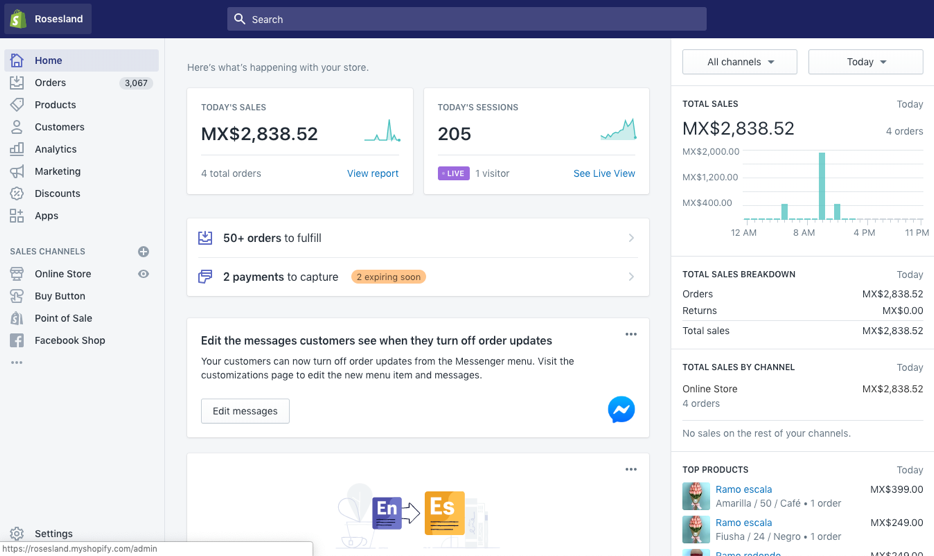
\includegraphics[width=0.9\textwidth]{shopify}
  \caption{Interfaz del administrador Shopify.}
\end{figure}